\documentclass{article}
\usepackage[utf8]{inputenc}
\usepackage[swedish]{babel}
\usepackage{authblk}
\usepackage[sorting=none]{biblatex}
\addbibresource{sources.bib}
\usepackage{graphicx}
\usepackage[T1]{fontenc}
\usepackage{ae}
\usepackage{multirow}
\usepackage[table]{xcolor}
\usepackage{pgfgantt}

    \title{\textbf{Larmsystem med MD407}\\ 
     \hspace{10cm}
     \hrule
    \hspace{10cm}
    Implementation av rörelsesensor, avståndsmätare och simulerad dörrenhet på MD407 mikrodator}
    
    \author{\\Alamin Alreda\\Sebastian Danckwardt\\Isac Holm\\Zaid Haj Ibrahim\\Edvin Svahn}

    \date{Oktober 2022}
    
    %LÄÖGGG TILL: handledare, e-post adresser, sektion
    
\begin{document}

\maketitle
\newpage
\tableofcontents
\newpage
\section*{Ordlista}
Lista över beteckningar som används i denna rapport.
\begin{description}


\item[Buss] En buss är en kommunikationsport som tillåter överföring av data i form av elektriska signaler.

\item[CAN] Controller Area Network är en databuss som tillåter kommunikation mellan mikrokontrollers. MD407 är bestyckad med två CAN bussar.

\item[CAN] Controller Area Network är en databuss som tillåter kommunikation mellan mikrokontrollers. Detta görs med två bussar som sitter på korten.

\item[GPIO] General Purpose Input Output är en anslutningsport på MD407 där olika logiska enheter kan anslutas för att ta emot eller skicka data.

\item[Knappsats] En extern periferienhet med 16 knappar som används för inmatning av data till mikrokontroller.

\item[Kopplingsplatta] En platta där logiska enheter kan anslutas med kablar via kopplingsstift.

\item[SW-18010] Vibrationssensor

\item[USART] Universal Synchronous/Asynchronous Reciever/Transmitter är kopplingen mellan MD407 och terminalen.

\end{description}
 \newpage

\setcounter{page}{1}
\section{Introduktion}

Under året 2021 anmäldes 72 884 inbrottsstölder i Sverige vilket pekar på att det finns ett tydligt behov av larmsystem i dagens samhälle.\cite{BRa} Trots den oro som finns i allmänheten för att ens egendom ska bli stulen så tillkännager endast 13 \% av unga mellan 23 och 35 år att de äger en larminstallation.\cite{MoFor} En av de största anledningarna till detta är kostnaden, 20 \% av de som saknar ett hemlarm anger att priset på installation är för högt.\cite{MoFor} Genom att skapa ett prisvärt larmsystem kan man erbjuda möjligheten till en tryggare tillvaro.

%NY INTRODUKTION ADDERAD

\subsection{Syfte}
Projektet syftar till att skapa ett lättanvändligt larmsystem med rimligt pris som ska förhindra inbrott och stöld. Detta då endast 29 \% av Sveriges befolkning innehavar ett larmsystem.\cite{SSF} Systemet kommer eventuellt att kunna installeras i byggnader och institutioner, vilket kommer att sänka inbrottet och ökar tryggheten.

%ÄNDRA: sista meningen skum ändra från "eventuellt att kunna installeras"

\subsection{Mål}
Målet med projektet är att konstruera ett larm och låssystem med två olika larmenheter. Den ena ska kunna upptäcka i fall en dörr står öppen, och den andra ska detektera rörelse och vibrationer. 
En central styrenhet ska utgöra den del av larmsystemet som har i uppgift att kommunicera med de fristående larmenheterna.
Detta ska möjliggöra centraliserad kontroll och kalibrering av flera periferienheter i ett större larmsystem.
Ytterligare en periferienhet ska simulera ett defekt larm som ska skicka data i överflöd till central enheten.

När den centrala styrenheten startar ska en förfråga skickas till de anslutna periferienheterna. Därpå svarar varje periferienhet med dess typ och konfiguration för att sedan tilldelas ett unikt ID. Dörrenheten ska inledningsvis larma lokalt med en röd lysdiod, om specifika krav nås meddelas den centrala styrenheten. Dörrlarmet larmar till centralenheten efter en bestämd tid. Avståndsmätare ska upptäcka ifall något passerar framför den på ett visst avstånd och vibrationssensor ska detektera rörelse. Det ska även vara möjligt att låsa in eller låsa upp dörren samt inaktivera dörrlarmet genom att mata in en fyrsiffrig kod på en knappsats ansluten till centralenhet.

%ÄNDRA: gör tydligt vad som är delmålen i projektet

\subsection{Arbetsmetod LÄGG TILL MER }
I arbetsmetod beskrivs hur .


\subsubsection{Process}
När gruppen började skriva kod för projektet delades den upp i två undergrupper som var och en arbetade självständigt med separata delar av projektet. 
Undergrupperna arbetade parallellt med varandra på distansmätaren och vibrationssensorn från början tills de var klara och sedan gick vidare till nästa del av projektet.
Vi genomförde också rigorösa tester när en funktion var färdig eller behövde testas genom att följa en testplan som hela gruppen enades om. 
Detta säkerställde att den nya koden integrerades väl med den befintliga koden och att den fungerade som det var tänkt.
Vi använde också ett versionshanteringsystem för att hålla reda på ändringar i koden och för att enkelt kunna återgå till en äldre version om något gick fel.
Projektgruppen hade också regelbundna möten med projektledaren,
där vi gick igenom vad vi hade gjort under föregående vecka samt vad vi arbetade med under den aktuella veckan och om vi hade några problem.
Detta hjälpte oss att hålla projektet på rätt spår och se till att vi gjorde goda framsteg.

%SKRIV OM / FLYTTA till efter teknisk beskrivning?

\newpage
\section{Teknisk beskrivning}
I det här kapitlet redogörs en teknisk beskrivning av systemet. 
I den tekniska bakgrunden beskrivs vad samtliga komponenter har för syfte.

Därefter ger Systemöversikt en övergripande förståelse för hur systemet är uppbyggt. Delsystem förklarar hur samtliga delarna är uppbyggda.

\subsection{Teknisk bakgrund}\\
%Vad är utgångspunkten för konstruktionsarbetet?
%välj en av följande stycken
I dagens samhälle har digitalisering en stor del av världens revolution och utveckling, en revolution att jämföra med industliersering i 1900. Begreppet digitalisering innebär att,med hjälp av teknik, förbättra människors livstill. Detta sker genom att omvandla beffintliga verksamhet till nya som är mer effiktiva och innovativa, exmpelvis ett larmsystem. 

Digitala larmsystem används för att upptäcka inbrott eller obehörigt inträde i privata fastigheter, industriella anläggningar samt militära skyddsobjekt. Larmsystem kan ha olika konstruktion beroende på säkerhetsbehov men samtliga system tillämpar flertal olika sensorer för att upptäcka inbrott. I fall en avvikelse upptäcks av en sensor ska larmet aktiverats och användare underrättas.

I konstruktionsarbetet är MD407-mikrokontroller den centrala komponenten. Detta är en laborationsdator med stabil hårdvara som har utvecklats i utbildningssyfte. Då datorn är utvecklad för utbildning finns det skydd mot ESD, felkopplingar och mekaniska påfrestningar vilket gör den lämpad för utveckling av prototypsystem.

För att MD407 ska kunna skicka och ta emot data från externa perifierienheter är den bestyckad med flera olika anslutningar som kan användas för detta. GPIO (General Purpose Input Output) lämpar sig för koppling med enklare periferienheter och är den anslutningen som används för kommunikation med Avståndsmätare samt Vibrationssensor (HC-SR04 respektive SW-18010P). Det finns 5 GPIO portar A-E, portarna har 16 kontaktstift vardera som kan konfigureras till att hantera indata eller utdata. Det finns även kontaktstift för ström samt jord som används av sensorerna.

Då åtskilliga MD407-mikrokontrollers behöver kommunicera med varandra är de bestyckade med två CAN portar, vilket möjliggör en loopback där samma mikrokontroller kan skicka meddelanden till sig själv vilket förenklar testning. MD407 ansluts via CAN bussarna med RJ-11 kablage.

%Vibrationssensorn går att köpa för ca 7 kr och en avståndsmätare för ca 50 kr.
%Lägg till några kablar och en bräda att koppla det på så blir det kanske runt ca 150 kr. 
%Det finns ingen prispunkt på MD407-korten på internet men liknande kort finns för överkant 150 kr.\\

%Med tre kort och lägsta möjliga sensorer kostar det ca 750 kr vilket är en engångssumma till skillnad från ett hemlarm på prenumeration kan kosta ca 250 kr i månaden \cite{Offerta}.
%Det betyder att du har tjänat in kostnaden efter ca 3 månader beroende på hur många komponenter du köper.\\

\subsection{Systemöversikt}

%\newpage 
\begin{figure}[h]
    \centering
    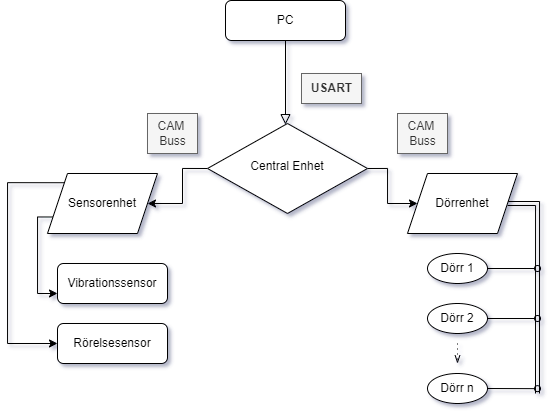
\includegraphics[scale=0.8]{Projektrapport/diagram.png}
    \caption {Blockschema av larmsystemet. Pilarna indikerar på GPIO-port koppling mellan dörrerna/sensorerna till MD-kort. Dubbel-pilar mellan dörenheten och dörrarna indikerar på att det finns en kopplingsplatta.}
    \label{fig:drawing}
\end{figure}

Systemet består i stort av tre delar, en centralenhet och två periferienheter, en dörrenhet och sensorenhet. 
Utöver dessa enheterna innehåller systemet övriga komponenter som bidrar till funktionalitet av systemet i sin helhet såsom tangentbord och 7-segmentdisplay. Ett MD407-kort används som en centralenhet för att koppla ihop olika komponenter beroende på deras funktion och uppgifter (figure 1).
Kommunikation mellan samtliga md-kort sker via en CAN-buss, medan kommunikation mellan centralenheten och PC sker över USART. \\
\\

Dörrenhet ska vara ansluten till en kopplingsplatta, på plattan ska det finnas lampor och en dörr-strömbrytare som läser av dörrens tillsånd.
Lamporna kommer lysa rött efter att dörren har varit öppen en viss tid eller grönt om inget larm har gått. 
Dörr-strömbrytarna kommer att simulera dörröppning eller dörrstängning. 
\\
Sensorenhet ska vara kopplades till en avståndsmätare (HC-SR04) och en vibrationssensor (SW-18010P). 
Avståndmätaren kommer att skicka en signal om avståndet har ändrats. 
På samma sätt kommer vibrationssensorn skicka en signal om den har känt av några vibrationer. \\

\begin{figure}[h]
    \centering
    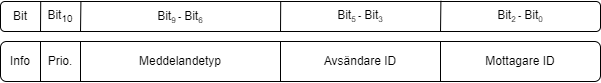
\includegraphics[scale=0.5]{Projektrapport/protokoll.png}
    \caption {Visuell framställning av Kommunikationsprotokoll}
    \label{fig:drawing}
\end{figure}


\subsection{Delsystem}
%gör beskrivning
Här beskrivs vad de olika delsystemen har för tekniska funktioner samt arbetsroller under utförandet av systemet. 

\subsubsection{Centralenhet}
Centralenheten kommunicerar ständigt med dörrenheten och sensorenheten över en CAN-buss, denna kommunikation kommer att omfatta ACK-, larm-, och konfigurationsmeddelanden. 
Dessutom ska centralenheten hantera all kommunikation mellan användaren och systemet genom USART. För att användaren ska få tillgång till systemet ska det korrekta lösenordet skrivas in. 
Därefter ska användaren kunna, för varje dörr, slå på eller av det centrala larmet, ändra tröskelvärdet, låsa eller låsa upp dörren. 
Utöver det ska användaren också kunna ändra tröskelvärdet för avståndsmätaren.

\begin{figure}[h]
    \centering
    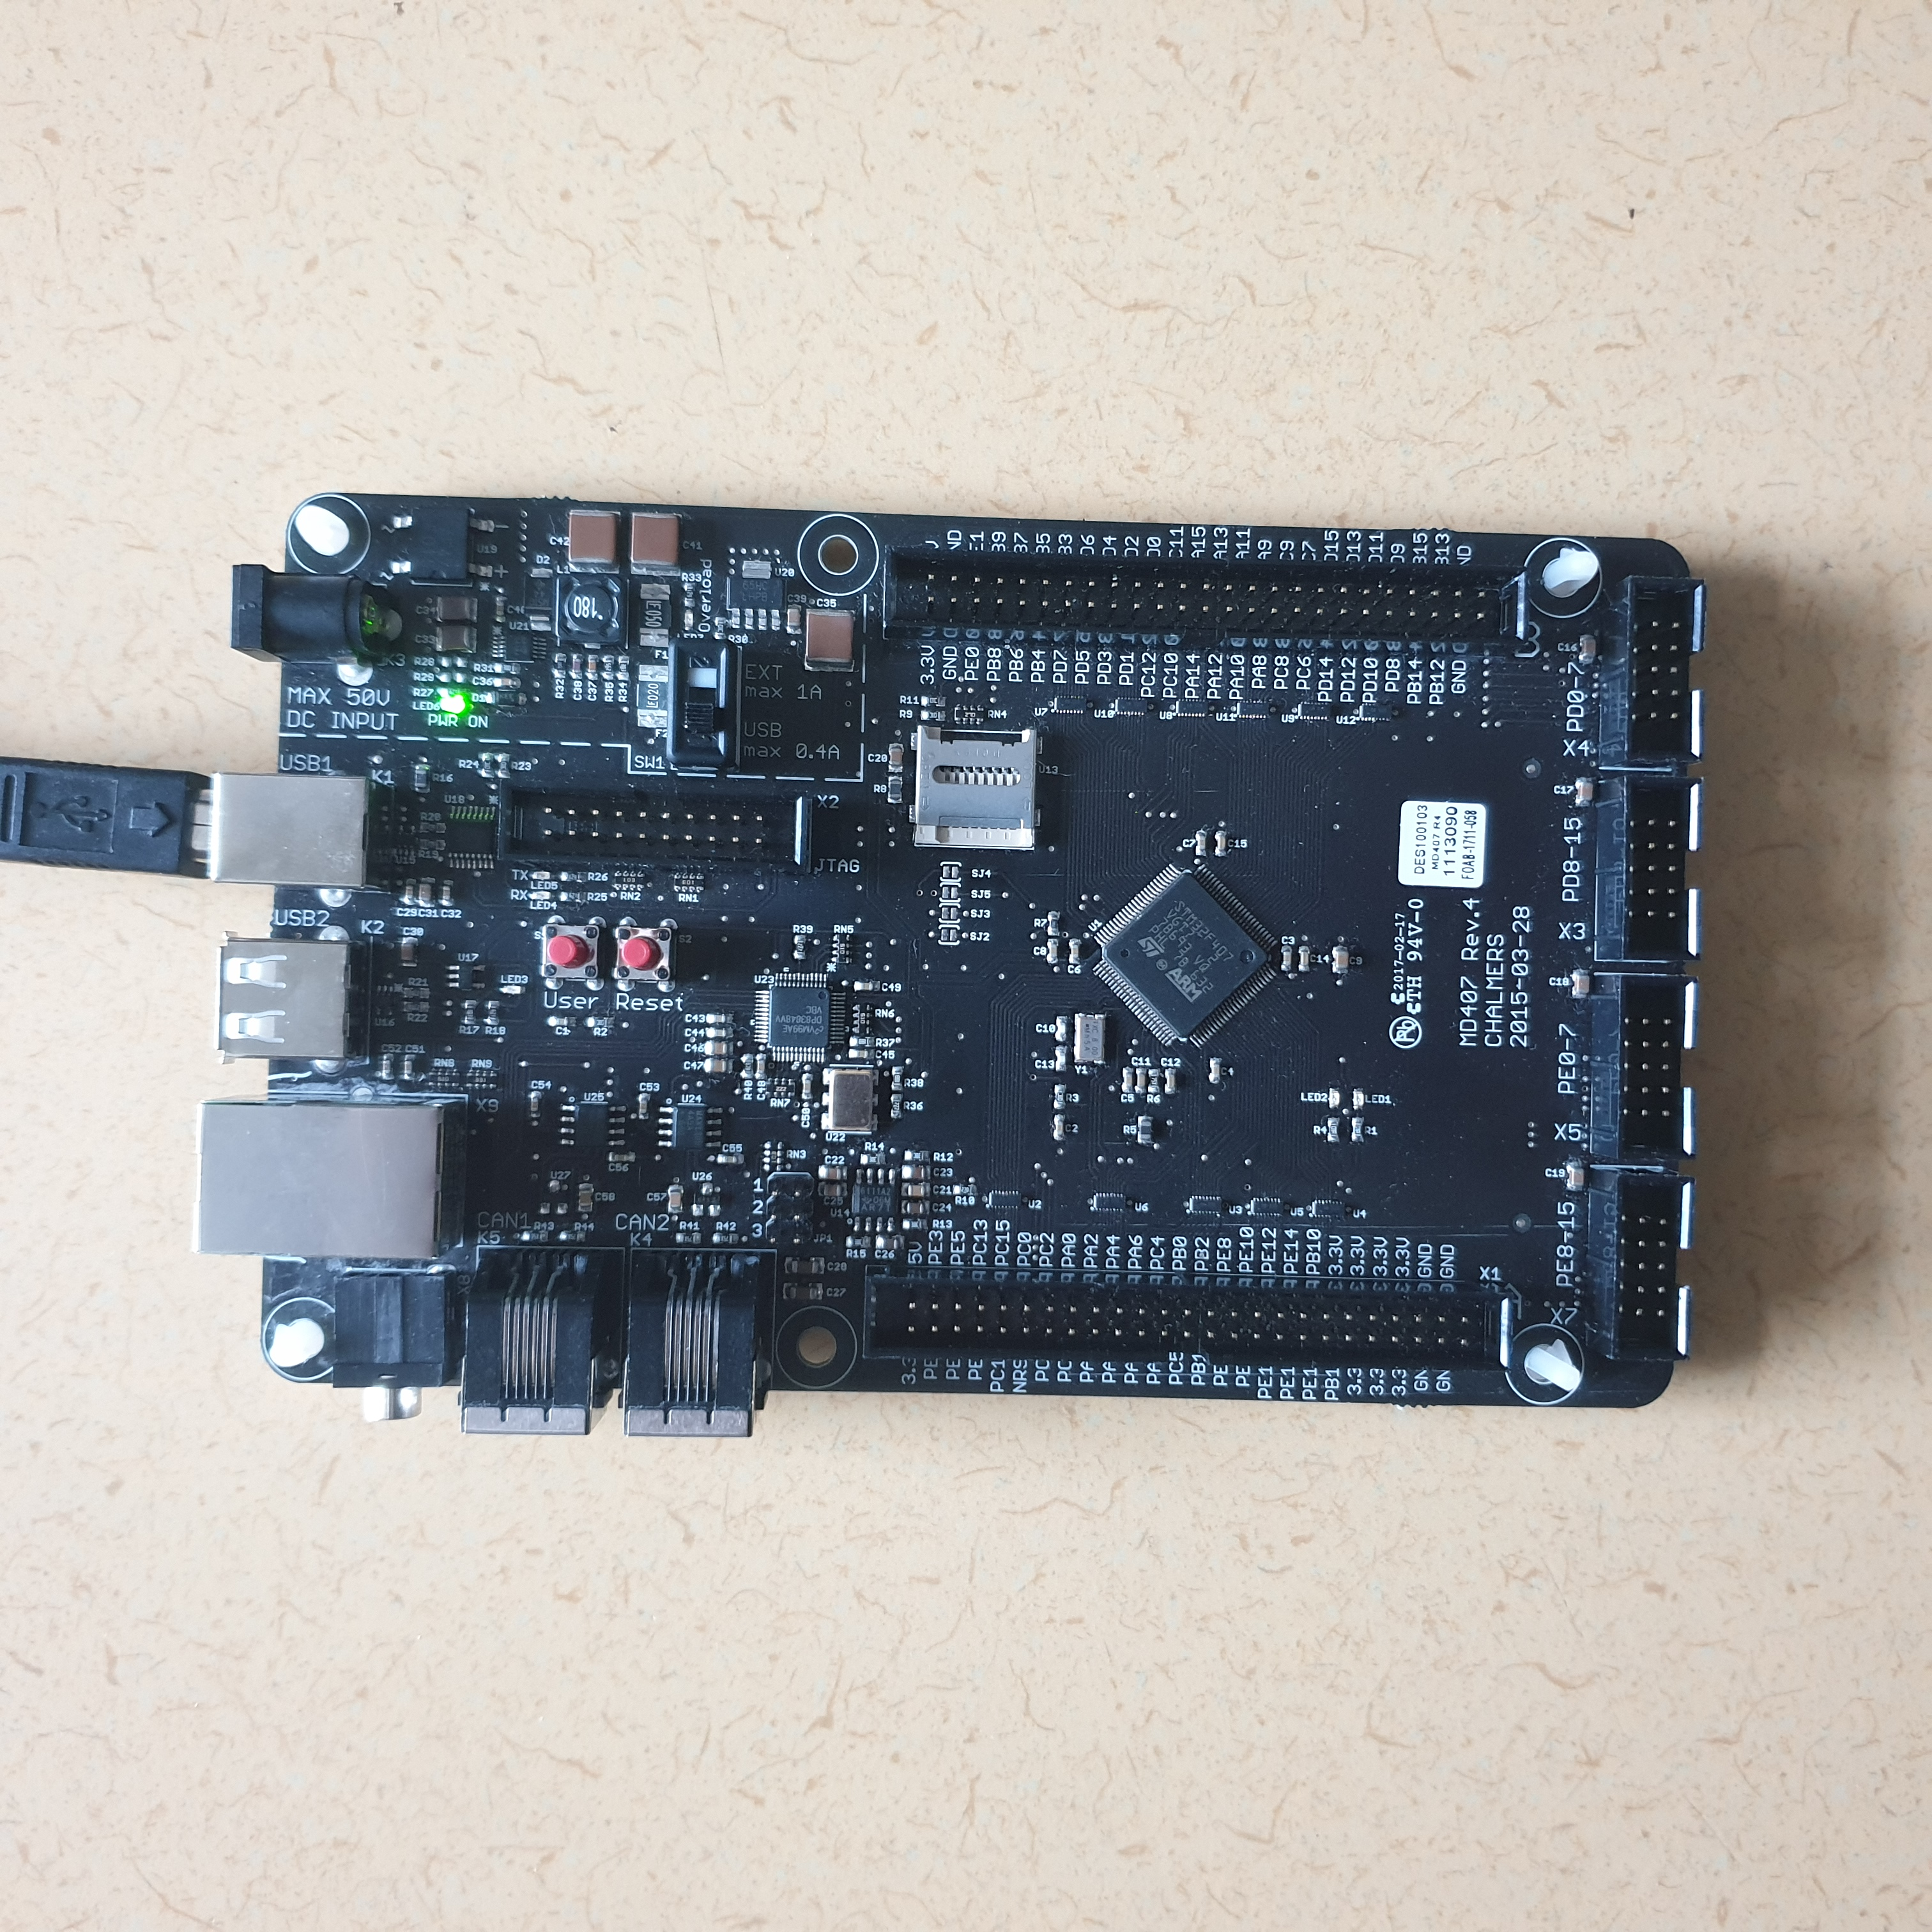
\includegraphics[scale=0.05]{Projektrapport/central.png}
    \caption {Hårdvaran som har funktionen som centralenhet}
    \label{fig:drawing}
\end{figure}

\subsubsection{Dörrenhet}

Dörrenheten kommer att vara kopplad till flera dörrar, där varje dörr kommer att vara kopplad till en grön lampa, en röd lampa och ett lås.Utöver det kommer varje dörr att ha sitt eget tröskelvärde som bestämmer när larmet ska gå av. 
När tiden har gått ett tröskelvärde kommer det lokala larmet att gå av och det kan man se genom att den röda lampan lyser. 
Efter två tröskelvärden kommer dörrenheten att skicka till centralenheten för att påställa störenheten. 
Om dörren är stängd ska den gröna lampan lysa medan det lokala och centrala larmet ska vara avstängda. 

\subsubsection{Sensorenhet}

Sensorenheten kommer att vara kopplad till två sensorer: avståndsmätare och vibrationssensor (HC-SR04 respektive SW-18010P).
Avståndsmätaren kommer att läsa av avståndet till ett objekt genom att skicka ultraljudssignaler och vänta på att få tillbaka ett eko. 
Mätningen av avståndet kommer att ske genom att räkna skillnaden i mikrosekunder mellan ultraljudssignaler och deras eko, därefter divideras tiden med 58 för att få avståndet i centimeter. 
Avståndet kommer att mättas kontinuerligt i intervaller av 60 millisekunder, om avståndet överstiger eller blir mindre än tröskelvärdet kommer det centrala larmet att gå.\\
\\
Sedan kommer även vibrationssensor att känna av vibrationer, ifall den känner av någon vibration kommer den att den skicka till centralenheten för att slå på det globala larmet.

\begin{figure}[h]
    \centering
    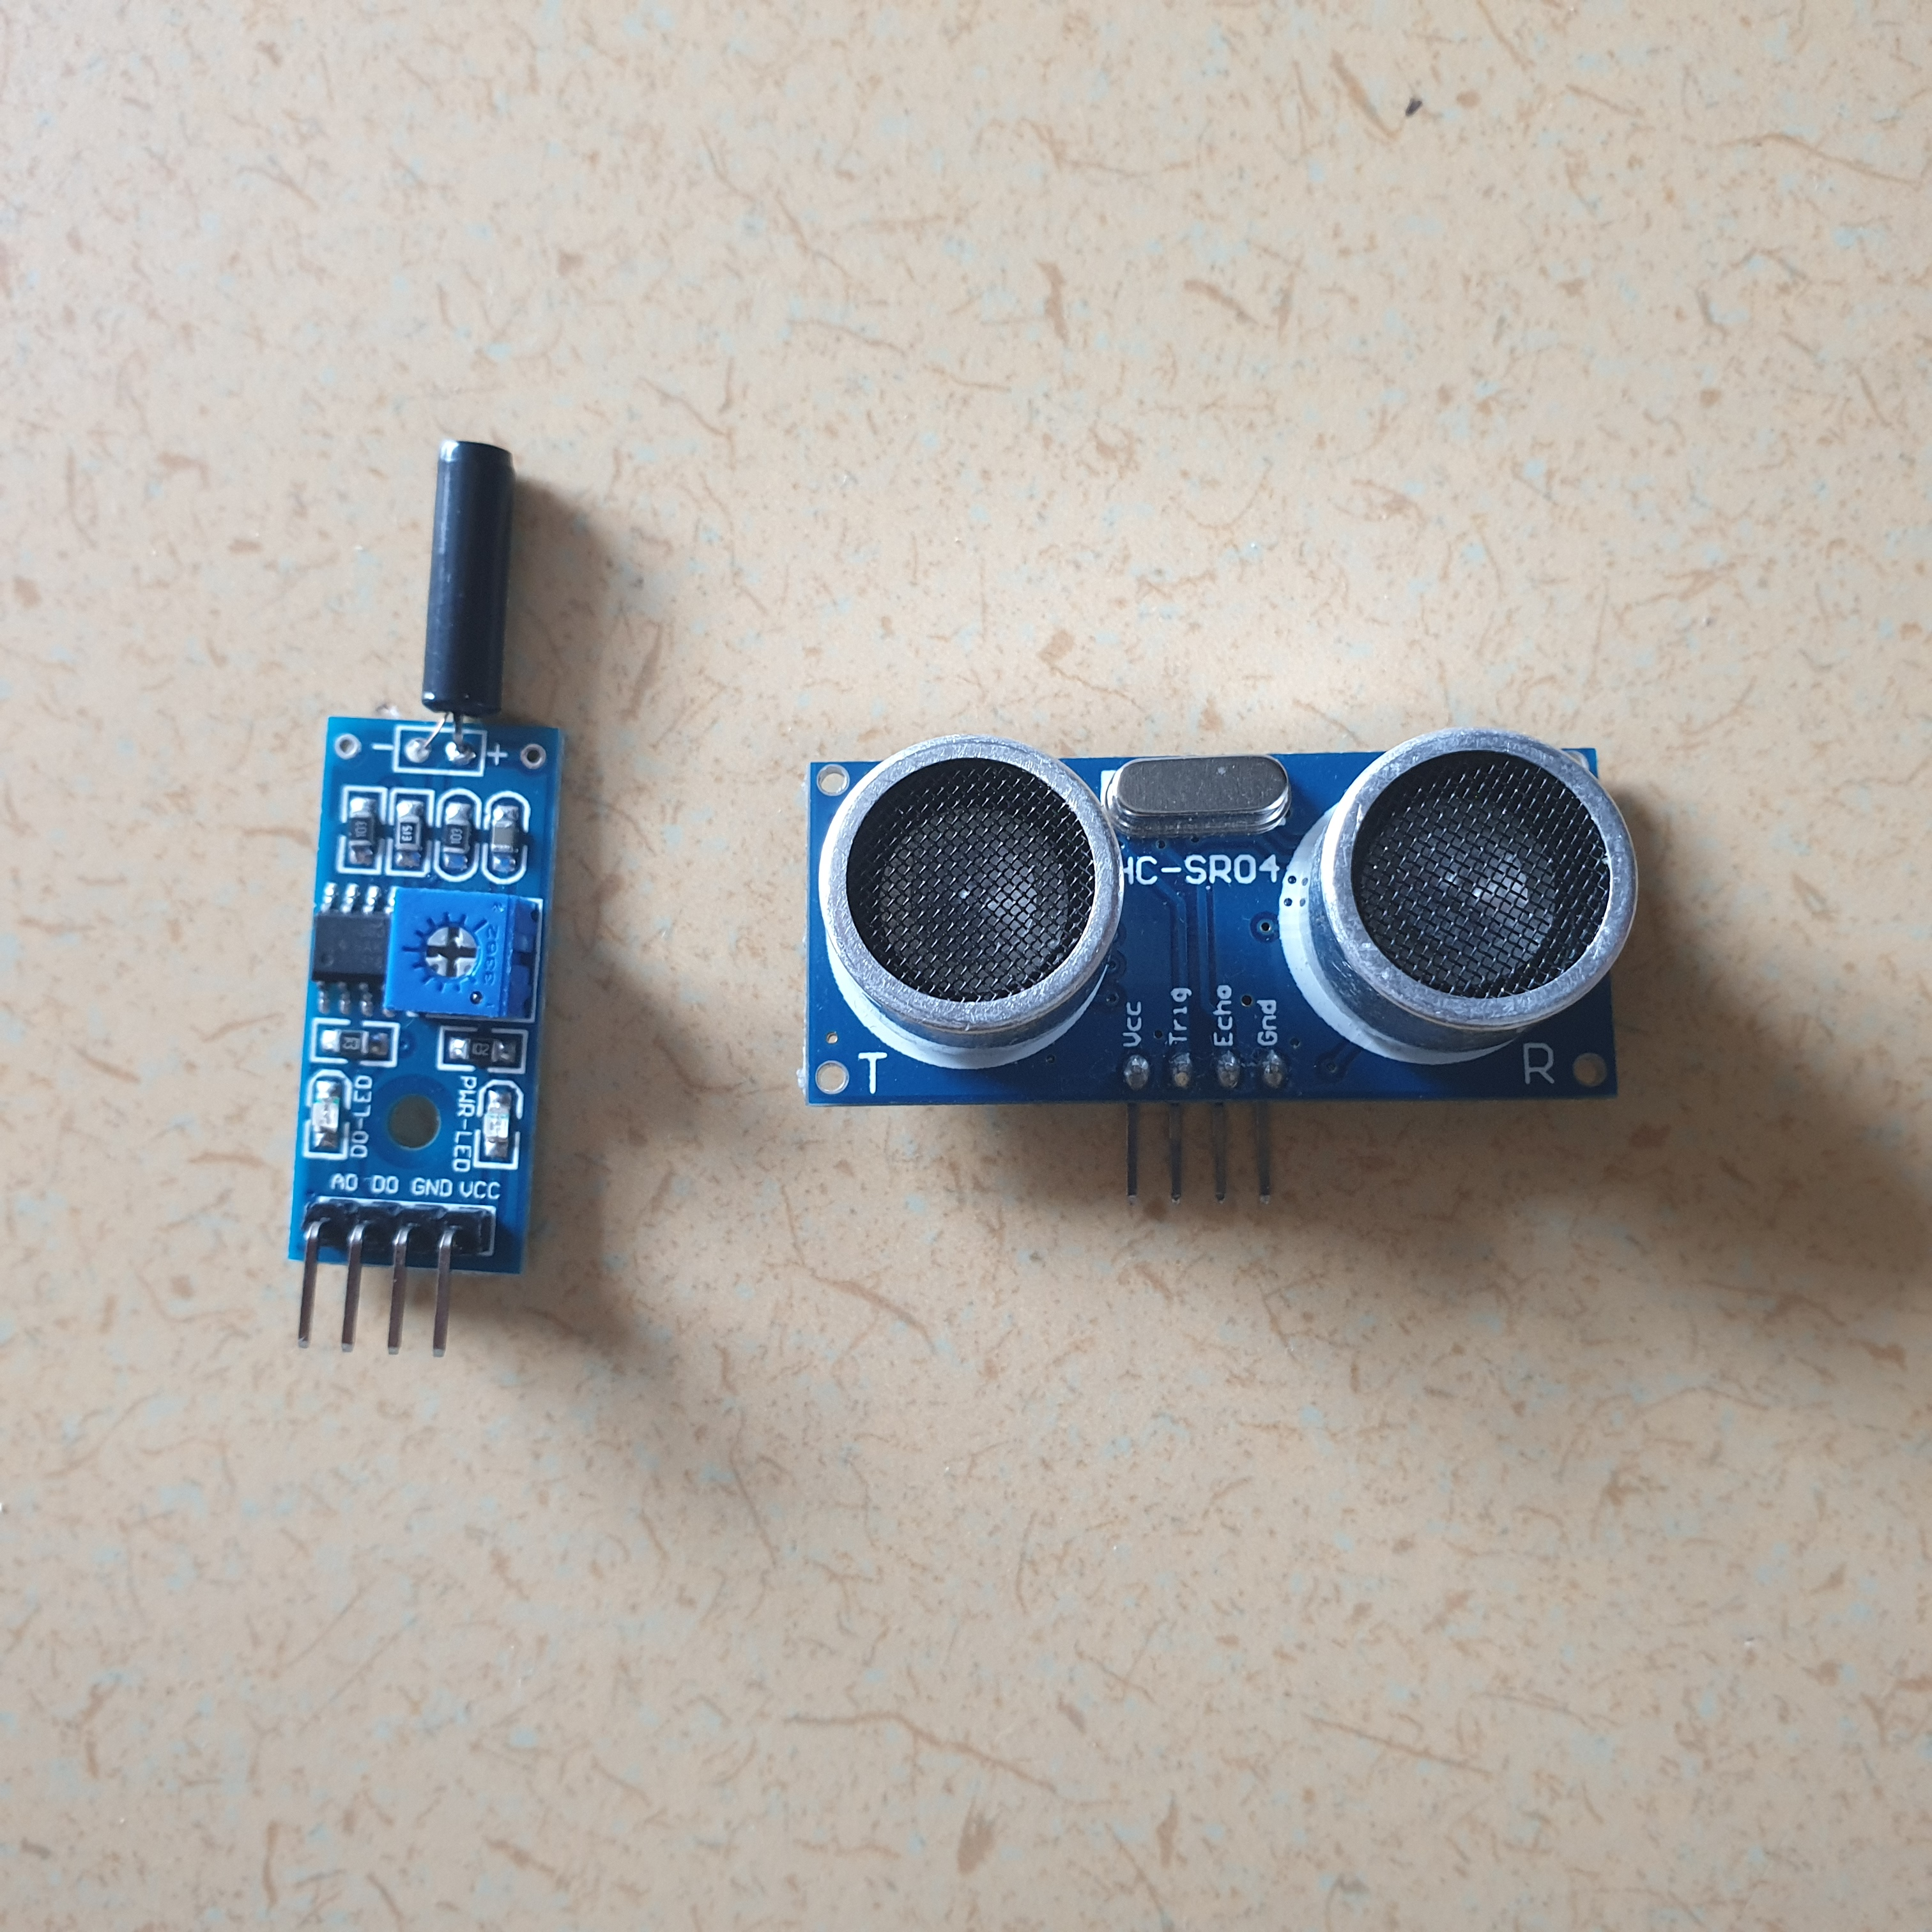
\includegraphics[scale=0.05]{Projektrapport/sensor.png}
    \caption {Hårdvaran till vänster är vibrationssensor, till höger är avståndsmätare}
    \label{fig:drawing}
\end{figure}
\subsubsection{Systemprotkoll}\\
Kommunikationsprotkollet är en 10-bit lång protokoll, vilket är uppdelat till fyra segment (figure 2). Högsta bit är tilldelade till bit-10, och lägsta bit är bit-0. Ett ställning av bit-10 innebär att detta meddelande får högsta prioritet och därmed viktigt att utföras först i fall det skulle bygga up datakö i CAN-bussen. Noll-ställning av samma bit innebär då motsatsen, vilket är att meddelandet får lägsta prioritet och kan därmed vänta med utförande. Bit 9 till och med bit 6 är reserverade till meddlandetypen som innehåller blandannat om meddelandet är ett begär att larma på eller av, eller bland annat information som föras mellan olika enheterna i regelbundet. Varje gång ett meddelande skickas, kommer bit-5 till och med bit-3 innehålla avsändaren ID, och bit2 till och med bit-0 ansvariga för mottagarens ID. 

\section{Resultat}
Detta avsnitt redovisar resultatet av genomförd verifiering av systemet och dess olika delar

\subsection{Mätning av avstånd}
Under utvecklingen av mjukvaran för avståndsmätaren har ett test skrivits för att observera vilket avståndet är det som räknas. Testet genfördes med hjälp av en linjal för att kontrollera att avståndsmätaren räknar rätt avstånd. Resultatet visade att att avstånddsmätaren kunde räkna precisa värden i centimeter. Ett ytterligare test genomfördes för att kontrollera att sensorenheten kommer att skicka ett larm när avståndet har understiget eller blivit större än tröskelvärdet. Testet genomfördes med hjälp av en linjal och resultatet visade att sensorenheten kommer att skicka ett larm när avståndet avviker från tröskelvärdet. 

\subsection{Mätning av vibrationer}
Den huvudsakliga uppgiften av vibrationsensorn är att larma när en vibration har inträffats, under testningen av sensorenheten har vi lyckats få ett larm när vibrationsensorn har skakats.


\subsection{Dörrlarm}
Dörrenhetens uppgift är att den, om en dörr är öppen, larmar lokalt när tiden har passerat ett tröskelvärde och larmar centralt när tiden har passerat två tröskelvärden. Under testningen av enheten har den uppfyllt de målen som krävdes.


\section{Slutsats och diskussion}
Med resultaten kan man konstatera att det går att skapa ett eget larm om man har möjlighet att införskaffa komponenterna.\\

Tyvärr så kan mycket problem uppstå ifall man väljer att skapa systemet själv.
För det första så måste man räkna med att få spendera mer tid för att programmera de olika delsystemen samt för att koppla ihop allting, för att inte tala om att bygga ett protokoll från grunden.
I fallet med kortet MD407 kan det bli begränsande vilka utvecklingsmiljöer som fungerar att använda felfritt då det inte finns så mycket dokumentation på just det kortet jämfört med kanske lite vanligare kort såsom en Arduino eller ett Raspberry Pi.\\

Fördelarna väger fortfarande tungt då det både är billigare att köpa in de diverse komponenterna och koppla själv än att köpa en prenumeration där installation ingår, 
samt ger en större valmöjlighet när det kommer till egenskaper. 
Man kan till exempel använda sig av en motor som man kopplar en avståndsmätare på för att kunna få den att snurra runt sin axel och på så sätt kunna få en kamera som kan se runt sig och få en bild av omgivningen i form av avstånd.

\newpage
\section{Källförteckning}
\printbibliography[heading=none]

\end{document}